\documentclass[12pt]{article}

\usepackage{mathptmx}
\usepackage{amsmath} % better math support
\usepackage{amssymb} %maths
\usepackage[utf8]{inputenc} %useful to type directly diacritic characters
\usepackage{graphicx}
\usepackage{times}
\usepackage{url}
\usepackage{color}
\usepackage{algorithm2e}
\usepackage{natbib}

\renewcommand{\topfraction}{1.00}
\renewcommand{\bottomfraction}{.7}
\renewcommand{\textfraction}{.0}
\renewcommand{\floatpagefraction}{.97}
\renewcommand{\dbltopfraction}{.97}
\renewcommand{\dblfloatpagefraction}{.97}
\setcounter{topnumber}{9}
\setcounter{bottomnumber}{9}
\setcounter{totalnumber}{20}
\setcounter{dbltopnumber}{9}

\title{Practical Data Analysis: Designing a Real-World Outlier Detector}
\author{Leland Wilkinson  \\
H2O.ai \\
Department of Computer Science, University of Illinois at Chicago. \\ 
email: \texttt{leland@h2o.ai} \\
\\
Erin LeDell \\
H2O.ai \\
email:\texttt{erin@h2o.ai}
}



\begin{document}

\maketitle

\begin{abstract}
Theory and practice do not always coincide in the world of real data analysis. This paper presents a new algorithm,  called $\mathtt{hdoutliers}$, for detecting multidimensional outliers. It is designed specifically to a) deal with a mixture of categorical and continuous variables, b) deal with the curse of dimensionality (many columns of data), c) deal with many rows of data, d) deal with outliers that mask other outliers, and e) deal consistently with unidimensional and multidimensional problems. Unlike ad hoc methods found in many machine learning papers, $\mathtt{hdoutliers}$ is based on a distributional model that allows outliers to be tagged with a probability. And unlike many methods found in the statistical literature, it presents opportunities for extending the problem to messy datasets.
\end{abstract} % end of abstract

\section{Introduction}
It is often said that data science is 90 percent data preparation and 10 percent data analysis. We can go on to say, in another wild guesstimate, that data analysis is 90 percent discovery and 10 percent modeling. Even when we have mapped our data to a rectangular matrix of real numbers, we cannot apply statistical or machine learning models without giving a lot of thought to violations of assumptions, missing values, outliers, and other threats to the validity of our inferences. Statisticians have understood this for many years. 

Practical data analysis involves more than investigating model assumptions, however. In many cases, there is a discrepancy between a theoretical statistical or machine learning model and what is needed to implement that model on real data. In practical data analysis we often encounter wide, deep, heterogeneous, sparse, or massive data that do not fit a standard model. In these cases, we need to encapsulate an analytic method in an extended algorithm designed to deal with these peculiar data structures. This effort is not part of what we normally call data preparation. Instead, it involves the analytic process itself. Unless we properly address this problem, we may not be able to find a valid answer to our analytic question.

We will use a common analytic question and an associated algorithm to illustrate our point: how do we find anomalies, specifically outliers, in a set of data? Despite more than a century of statisticians offering answers to this question, none of the traditional statistical or machine learning outlier detection methods are of much use when applied to most real data. They are all predicated on restrictive assumptions that do not apply to most practical situations. 

The difficulties we face in devising a practical method are several. In working with real data, we often encounter:
\begin{itemize}
\setlength\itemsep{0em}
\item too many columns of data (the curse of dimensionality)
\item too many rows of data (scalability)
\item sparse data
\item a mixture of categorical and continuous variables
\item missing or undefined values
\item outliers that mask other outliers
\end{itemize}

Before showing how we may deal with some of these problems, we will summarize related work on outlier detection.

\section{Related Work}
There are several excellent books and surveys on outliers \citep{BarnettLewis,Hawkins,RousseeuwLeroy,thode2002testing,HadiSimonoff,IglewiczHoaglin,AnscombeOutliers,AggarwalOutliers,ChandolaBanerjeeKumar,HodgeOutliers}. We summarize the basic approaches in this section.

\subsection{Univariate Outliers}
The detection of outliers in the observed distribution of a single variable spans the entire history of outlier detection. It spans this history not only because it is perhaps the simplest formulation of the problem, but it also has numerous practical applicatons.

\subsubsection{The Distance from the Center Rule}
The word {\it outlier} implies lying at an extreme end of a set of ordered values -- far away from the center of those values. The modern history of outlier detection emerged with methods that depend on a measure of centrality and a measure of distance from that measure of centrality. As early as the 1860's, Chauvenet \citep{BarnettLewis} judged an observation to be an outlier if it lies outside the lower or upper $1/(4n)$ points of the Normal distribution. \cite{BarnettLewis} document many other early rules that depend on the Normal distribution but fail to distinguish between population and sample variance.

\cite{Grubbs}, in contrast, based his rule on the sample moments of the Normal:
\begin{equation*}
G = {{\max\limits_{1 \leq i \leq n} \vert x_i - \bar{x} \vert} \over s}\\
\end{equation*}
where $\bar{x}$ and $s$ are the sample mean and standard deviation, respectively.

Grubbs referenced $G$ against the $t$ distribution in order to spot an upper or lower outlier:

\begin{equation*}
G > {{n - 1} \over{\sqrt{n}}} \sqrt{t^2_{\alpha / (2n), n-2}\over{n-2 + t^2_{\alpha / (2n), n-2}}}
\end{equation*}

If one knows that the values on a variable are sampled randomly from a Normal distribution and if the estimates of location and scale are unbiased and if one wishes to detect only the largest absolute outlier, it is a valid test.

Unfortunately, the usual sample estimates of the mean and standard deviation are not robust against outliers. So we have a circularity problem. We assume a null distribution (say, the Normal), estimate its parameters, and then use those estimates to test whether a point could have plausibly come from that distribution. But if our alternative hypothesis is that it doesn't (the usual case), then the outlier should not be included in the estimation. \cite{BarnettLewis} discuss this problem in more detail, where they distinguish {\it inclusive} and {\it exclusive} methods. They, as well as \cite {RousseeuwLeroy}, also discuss robust estimation methods for overcoming this circularity problem.

Barnett and Lewis discuss other detection methods for non-Normal distributions. The same principals apply in these cases, namely, that the sample is random, the population distributions are known and that the parameter estimates are unbiased.

\subsubsection{The Box Plot Rule}
A box-plot graphically depicts a batch of data using a few summary statistics called {\it letter values} \citep{EDA,FriggeHoaglinIglewicz}.  The letter values in Tukey's original definition are the median and the {\it hinges} (medians of the upper and lower halves of the data). The hinge values correspond closely, but not necessarily, to the lower quartile (Q1) and the upper quartile (Q3). Tukey called the difference between the hinges the {\it Hspread}, which corresponds closely to the quantity Q3--Q1, or the Inter Quartile Range (IQR). In Tukey's version of the box-plot (see the upper panel of Figure~\ref{fig:teaser}), a box is drawn to span the {\it Hspread}. The median is marked inside the box. Whiskers extend from the edges of the box to the farthest upper and lower data points ({\it Adjacent values}) inside the so-called {\it inner fences}. The upper inner fence is the \\
\begin{equation*}
upper hinge + 1.5 \times Hspread
\end{equation*}
and the lower inner fence is the \\
\begin{equation*}
lower hinge - 1.5 \times Hspread
\end{equation*}

Any data point beyond the {\it Adjacent values} is plotted as an outlying point. \footnotemark

\footnotetext{Few statistics packages produce box plots according to Tukey's definition \citep{FriggeHoaglinIglewicz}. Surprisingly, the boxplot function in the core {\it R} package does not, despite its origin in Tukey's group at Bell Laboratories.}

Tukey designed the box plot (he called it a {\it schematic plot}) to be drawn by hand on a small batch of numbers. The whiskers were designed not to enable outlier detection, but to locate the display on the interval that supports the bulk of the values. Consequently, he chose the {\it Hspread} to correspond roughly to three standard deviations on normally distributed data. This choice led to two consequences: 1) it doesn't apply to skewed distributions, which constitute the instance many advocates think is the best reason for using a box plot in the first place, and 2) it doesn't include sample size in its derivation, which means that the box plot will falsely flag outliers on larger samples. As \cite{Dawson} shows,  ``regardless of size, at least 30\% of samples drawn from a normally-distributed population will have one or more data flagged as outliers.'' The top panel of Figure~\ref{fig:teaser} illustrates this problem for a sample of 100,000 Normally distributed numbers. Thousands of points are denoted as outliers in the display.

\cite{HoaglinIglewiczTukey} and \cite{HoaglinIglewicz} modified Tukey's definition to include $n$ as a parameter, thus making the boxplot useful at least for symmetric distributions. To deal with the skewness problem, \cite{HubertVandervieren} and others have suggested modifying the fences rule by using a robust estimate of skewness. By contrast, Tukey's approach for this problem involved transforming the data through his {\it ladder of powers} \cite{EDA} before drawing the box plot.

The Letter-Value-Box-Plot \citep{letter-value-box-plot} was designed to deal with both problems. The authors compute additional letter values (splitting the splits) until a statistical measure of fit is satisfied. Each letter-value region is represented by a rectangle. The lower panel of Figure~\ref{fig:teaser} shows the result. On the same 100,000 Normal variables, only two points are identified as outliers.

\begin{figure}[h]
\centering
\includegraphics[width=10cm]{figures/boxes.pdf}
\caption{ \label{fig:teaser} Outliers revealed in a box plot \citep{EDA} and letter values box plot \citep{letter-value-box-plot}. These plots are based on 100,000 values sampled from a Gaussian (Standard Normal) distribution. By definition, the data contain no probable outliers, yet the ordinary box plot shows thousands of outliers. This example illustrates why ordinary box plots cannot be trusted to discover probable outliers.}
\end{figure}

\subsubsection{The Gaps Rule}
The gaps rule looks for outliers that are separated from other points instead of from a measure of central location. A simple example illustrates. Suppose we give a test to 100 students and find the mean score is 50 and the standard deviation is 5. Among these students, we find one perfect score of 100. The next lower score is 65. We might be inclined to suspect the student with a score of 100 is a genius or a cheat. On the other hand, if the perfect score is at the top of a chain of scores spaced not more than 5 points apart (assuming the same mean and standard deviation overall), we might be less suspicious. Classical outlier tests would not discriminate among these possibilities.

 \cite{DixonOutlierTest} developed an outlier test based on the gap between the largest point and the second largest point, standardized by the range of scores. His test was originally based on a normal distribution, but in subsequent publications, he developed nonparametric variations. Dixon tabulated percentage points for a range of $Q$ statistics.

\begin{equation*}
Q = {{x_n - x_{n-1}} \over {x_n - x_1}}
\end{equation*}

\cite{EDA} considered the more general question of identifying gaps anywhere in a batch of scores. \cite{WainerSchacht} adapted Tukey's gapping idea for a version of the test that weighted extreme values more than middle ones. They derived an approximate $z$ score that could be used to test the significance of gaps.

\cite{BurridgeTaylor} developed an outlier test based on the extreme-value distribution of gaps between points sampled from the Exponential family of distributions. This family is quite large (including the Normal, Exponential, Gamma, Beta, Bernoulli, Poisson, and many others). 

\subsection{Multivariate Outliers}
\subsubsection{Mahalanobis Distance}
The squared Mahalanobis distance ($D^2$) of a multidimensional point $\mathbf{x}$ from the centroid of a multivariate Normal distribution described by covariance matrix $\Sigma$ and centroid $\boldsymbol{\mu}$ is

\begin{equation*}
D^2 = (\mathbf{x}- \boldsymbol{\mu})'\Sigma ^{-1}(\mathbf{x}- \boldsymbol{\mu})
\end{equation*}
Figure~\ref{fig:Mahalanobis} shows how this works in two dimensions. The left panel shows a bivariate normal distribution with level curves inscribed at different densities. The right panel shows the same level curves as horizontal slices through this mountain. Each is an ellipse. Distance to the centroid of the ellipses is measured differently for different directions. The weights are determined by the covariance matrix $\Sigma$. If  $\Sigma$ is an identity matrix, then $D^2$ is equivalent to squared Euclidean distance.

\begin{figure}[h]
\centering{\includegraphics[width=250pt]{figures/Mahalanobis.pdf}}
\caption{\label{fig:Mahalanobis} Mahalanobis Distance. The left panel shows a bivariate Normal distribution. The right shows level curves for that distribution. Each curve corresponds to a value of $D^2$.}
\end{figure}
  
The squared distance in the above formula is a chi-square variate. This means that, if the assumption of Normality is met, $D^2$ can be tested against a chi-square distribution with $p$ degrees of freedom. As with univariate outlier tests based on a Normality assumption, this test is valid if the assumption of multivariate Normality is met. Unfortunately, this is seldom true for real data and, furthermore, estimates of the covariance matrix and centroid are far from robust. Consequently, this outlier test has limited applicability.

\cite{RousseeuwVanZomeren} introduce a robust Mahalanobis Distance estimator that can be used to overcome some of these problems. \cite{Stahel} and \cite{Donoho} have developed a similar estimator with a high breakdown point. In both cases, the computations are intensive and require additional designs to allow them to scale to big data.

\subsubsection{Multivariate Gap Tests} 
Multivariate data do not have a simple ordering for computing gaps between adjacent points. There have been several attempts at getting around this problem. \cite{Rohlf} proposed using the edge lengths of the geometric minimum spanning tree (MST) as a single distribution measure. Assuming these edges follow a gamma distribution, one could construct a gamma probability plot on them or examine the upper tail for judgments on outliers. There are problems with this method, however, when variates are correlated \citep{CaroniPrescott}. Similar methods based on the MST have been proposed \citep{LinMST,JohnVictor}, but they suffer from the same problem.

\subsubsection{Clustering} 
A popular multivariate outlier detection method has been to cluster the data and then look for any points that are far from their nearest cluster centroids \citep{ZahnClustering, JiangOutlierClustering,OutlierClustering,Jobe}. This method works reasonably well for moderate-size datasets with a few singleton outliers. Most clustering algorithms do not scale well to larger datasets, however. 

A related approach, called Local Outlier Factor (LOF) \citep{BreunigLOF}, is derived from density-based clustering. Like DBSCAN clustering \citep{DBSCAN},  it is highly sensitive to the choice of input parameter values and doesn't scale well.

Most importantly, clustering outlier methods are not based on a probability model (see \cite{FraleyRaftery} for an exception) so they are susceptible to false negatives and false positives. We will show one remedy in Section 3.3.2.

\section{A New Multivariate Outlier Algorithm}
A new algorithm $\mathtt{hdoutliers}$ is designed to meet several criteria at once:
\begin{itemize}
\item It allows us to identify outliers in a mixture of categorical and continuous variables.
\item It deals with the curse of dimensionality by exploiting random projections for large $p$ (number of dimensions).
\item It deals with large $n$ (number of points) by exploiting a one-pass algorithm to compress the data.
\item It deals with the problem of $masking$ \cite{BarnettLewis}, in which clusters of outlying points can elude detection by traditional methods.
\item It works for both single-dimensional and multi-dimensional data.

\end{itemize}
\subsection{The Algorithm}

\begin{enumerate}
\item If there are any categorical variables in the dataset, convert each categorical variable to a continuous variable by using Correspondence Analysis \cite{CA}.
\item If there are more than 10,000 columns, use random projections to reduce the number of columns to $p = 4 \log{n} / (\epsilon^2/2 - \epsilon^3/3)$, where $\epsilon$ is the error bound on squared distances.
\item Normalize the columns of the resulting $n$ by $p$ matrix $X$.
\item Let $row(i)$ be the $i$th row of $X$.
\item Let $radius = .1 / (\log{n})^{1/p}$.
\item Initialize $exemplars$, a list of exemplars with initial entry $[row(1)]$.
\item Initialize $members$, a list of lists with initial entry $[1]$; each exemplar will eventually have its own list of affiliated member indices.
\item Now do one pass through $X$:\\
\begin{algorithm}[h]
 \ForAll{$row(i)$, $i = 1, \dots, n$} {
 $d$ = distance to closest exemplar, found in $exemplars(j)$\\
\eIf {$d < radius$} {
add $i$ to $members(j) list$\\
}  {
add $row(i)$ to $exemplars$\\
add new list to $members$, initialized with $[i]$\\
 }
 }
\end{algorithm}
\item Now compute nearest-neighbor distances between all pairs of exemplars in the $exemplars$ list.
\item Fit an Exponential distribution to the upper tail of the nearest-neighbor distances and compute the upper $1 - \alpha$ point of the fitted cumulative distribution function (CDF).
\item For any exemplar that is significantly far from all the other exemplars based on this cutpoint, flag all entries of $members$ corresponding to $exemplar$ as outliers.
\end{enumerate}

\subsection{Comments on the Algorithm}

\begin{enumerate}
\item Correspondence Analysis (CA) begins by representing a categorical variable with a set of dummy codes, one code (1 or 0) for each category. These codes comprise a matrix of 1's and 0's with as many columns as there are categories on that variable. We then compute a principal components decomposition of the covariance matrix of the dummy codes. This analysis is done separately for each of $k$ categorical variables in a dataset. CA scores on the rows are computed on each categorical variable by multiplying the dummy codes on that row's variable times the eigenvectors of the decomposition for that variable. \footnotemark
\item The \cite{JohnsonLindenstrauss} lemma states that if a metric on $X$ results from an embedding of $X$ into a Euclidean space, then $X$ can be embedded  in $R^p$ with distortion less than $1 + \epsilon$, where $p \sim O(\epsilon^2 \log n)$. Remarkably, this embedding is achieved by projecting onto a $p$-dimensional subspace using random Gaussian coefficients. Because our algorithm depends only on a similarity transformation of Euclidean distances, we can logarithmically reduce the complexity of the problem through random projections and avoid the curse of dimensionality. The number of projected columns based on the formula in this step was based on $\epsilon = .2$ for the analyses in this paper. The value 10,000 is the lower limit for the formula's effectiveness in reducing the number of dimensions when $\epsilon = .2$.
\item $X$ is now bounded by the unit (hyper) cube.
\item A $row$ represents a $p$-dimensional vector in a finite vector space.
\item The value of $radius$ is designed to be well below the expected value of the distances between $n(n-1)/2$ pairs of points distributed randomly in a $p$ dimensional space.
\item The $exemplars$ list contains a list of row values representing clusters of points.
\item The $members$ list of lists contains one list of indices for each exemplar that point to rows represented by that exemplar.
\item The Leader algorithm \citep{ClusteringAlgorithms} in this step creates clusters in one pass through the data. It is equivalent to centering balls in $p$ dimensional space on points considered to be exemplars. Unlike $k$-means clustering, the Leader algorithm centers clusters on actual data points rather than on centroids and it involves only one pass through the data. In rare instances, the resulting clusters can be dependent on the order of the data, but not enough to affect the identification of outliers because of the large number of clusters produced. We are characterizing a high-dimensional density by covering it with many small balls. 
\item The number of clusters resulting from $radius$ applied even to large numbers of data points is small enough to allow the simple brute-force algorithm for finding nearest neighbors.
\item We use a modification of the \cite{BurridgeTaylor} algorithm due to \cite{SchwarzOutliers}. For all examples in this paper, $\alpha$ (the critical value) was set to .05.
\item Flagging all members of an outlying cluster means that this algorithm can identify outlying sets of points as well as outlying singletons.
\end{enumerate}
\footnotetext{Computing the decomposition separately for each categorical variable is equivalent to doing an MCA separately for each variable instead of pooling all the categorical variable dummy codes into one matrix.}


\subsection{Validation}
We validate $\mathtt{hdoutliers}$ by examining its performance with regard to 1) false positives and 2) false negatives. If the claims for the algorithm are true, then we should expect it 1) to find outliers in random data not more than $100 \alpha$ percent of the time and 2) not to miss outliers when they are truly due to mixtures of distributions or anomalous instances.

\subsubsection{False Positives}
\begin{itemize}
\setlength\itemsep{0em}
\item Table 1 contains results of a simulation using random distributions. The entries are based on 1,000 runs of $\mathtt{hdoutliers}$ on normally distributed variables with $\alpha$ (the critical value) set to .05. The entries show that $\mathtt{hdoutliers}$ is generally conservative. 
\item The results were similar for random Uniform variables. 
\end{itemize}

\begin{table}
 \caption{\label{errors} Empirical level of $\mathtt{hdoutliers}$ test based on null model with Gaussian variables and critical value $\alpha=.05$.}
 \scriptsize
 \begin{center}
   \begin{tabular}{lrrrr}
      & {\bf p=1} & {\bf p=5} & {\bf p=10} & {\bf p=100}\\
      
     {\bf n=100} & .011 & .040 & .018 & .012\\
     {\bf n=500} & .015 & .035 & .027 & .020\\
     {\bf n=1000} & .017 & .045 & .027 & .024\\
   \end{tabular}
 \end{center}
\end{table}
\subsubsection{False Negatives}
\begin{itemize}
\setlength\itemsep{0em}
\item Figure~\ref{fig:inliers} shows that $\mathtt{hdoutliers}$  identifies the inlier in the center of both one-dimensional and two-dimensional configurations.

\item Table 2 shows that $\mathtt{hdoutliers}$  identifies the outlier in a table defined by two categorical variables. The data consist of two columns of strings, one for \{A,B,C,W\} and one for \{A,B,C,X\}. There is only one row with the tuple $\langle W,X \rangle$. The $\mathtt{hdoutliers}$ also handles mixtures of categorical and continuous variables.
\end{itemize}

\begin{figure}[h]
\centering{\includegraphics[width=250pt]{figures/inliers.pdf}}
\caption{\label{fig:inliers} Inlier datasets; $\mathtt{hdoutliers}$ correctly identifies the inliers.}
\end{figure}

\begin{table}[h]
 \caption{\label{crosstab} Crosstab with an outlier (red entry)}
 \scriptsize
 \begin{center}
   \begin{tabular}{ccccc}
      & {\bf A} & {\bf B} & {\bf C} & {\bf X}\\

     {\bf A} & 100 & 0 & 0 & 0\\
     {\bf B} & 0 & 100 & 0 & 0\\
     {\bf C} & 0 & 0 & 100 & 0\\
     {\bf W} & 0 & 0 & 0 & \color{red}{\bf 1}\color{black}\\
   \end{tabular}
 \end{center}
\end{table}

\section{Visualization}
This section illustrates the adaptability of $\mathtt{hdoutliers}$ to a variety of applications. First, however, we document the shortcomings of popular visualization methods for identifying multivariate outliers.

\subsection{Low-dimensional visualizations cannot be used to discover multivariate outliers}
There have been many outlier identification proposals based on looking at axis-parallel views or low-dimensional projections (usually 2D) that are presumed to reveal high-dimensional outliers (e.g., \cite{Kandogan,Hinneburg,Kandogan:2001:VMC:502512.502530,KriegelKrogerSchubertZimek}). This approach is infeasible. Figure~\ref{fig:mahal} shows why. The data are samples from a multivariate Normal distribution. The left panel plot illustrates the problem for two dimensions. The figure incorporates a 95 percent joint confidence ellipse based on the sample distribution of points. Two points are outside this ellipse. The red point on the left is at the extreme of both marginal histograms. But the one on the right is well inside both histograms. Examining the separate histograms would fail to identify that point. 

The right panel plot shows the situation for three dimensions. The three marginal 2D plots are shown as projections onto the facets of the 3D cube. Each confidence ellipse is based on the pairwise plots. The red outlying point in the joint distribution is inside all three marginal ellipses. The 2D scatterplots fail to reveal the 3D outlier. The situation gets even worse in higher dimensions.

Some authors have proposed methods for finding low-dimensional views based on projection pursuit or ad hoc projections (e.g., \cite{BreabanLuchian,OutlierPP}). This approach is relatively ineffective for visualizing outliers in higher-dimensional datasets because many projections are required to discriminate outliers. Furthermore, most outlier-seeking projection methods are impractical on large datasets.

\begin{figure}[h]
\centering{\includegraphics[width=260pt]{figures/mahal2D3D.pdf}}
\caption{\label{fig:mahal} 2D (left) and 3D (right) joint outliers. The figures show why lower-dimensional projections cannot be used to discern outliers.}
\end{figure}

Parallel coordinates have been advocated for the purpose of outlier detection \citep{Novotny:2006:OFV:1187627.1187805}. Figure~\ref{fig:parallelcoordinates} shows why this is infeasible. The figure contains a parallel coordinates display on four variables from the Adult dataset in the UCI dataset repository \citep{adult}. The $\mathtt{hdoutliers}$ algorithm discovered two outliers out of 32,561 cases. The profiles appear to run through the middle of the densities even though they are multivariate outliers. Although parallel coordinates are generally useless for discovering outliers, they can be useful for inspecting outlier profiles detected by a statistical algorithm.

\begin{figure}[h]
\centering{\includegraphics[width=250pt]{figures/adult.pdf}}
\caption{\label{fig:parallelcoordinates}  Parallel coordinates plot of five variables from the Adult dataset in the UCI data repository. The red profiles are multivariate outliers.}
\end{figure}

\subsection{Using statistical algorithms to highlight outliers in visualizations}
While visualizations cannot be used to detect multidimensional outliers, they are invaluable for inspecting and understanding outliers detected by statistical methods. This section covers a variety of visualizations that lend themselves to outlier description.

\subsubsection{Time Series Outliers}
Detecting time series outliers requires some pre-processing. In particular, we need to fit a time series model and then examine residuals. Fitting parametric models like ARIMA \citep{BoxJenkins} can be useful for this purpose, but appropriate model identification can be complicated. A simpler approach is to fit a nonparametric smoother. The example in Figure~\ref{fig:snow} was fit by a kernel smoother with a biweight function on the running mean. The data are measurements of snowfall at a Greenland weather station, used in \cite{GoG}. The outliers (red dots) are presumably due to malfunctions in the recording equipment.

Computing outlying series for multiple time series is straightforward with the $\mathtt{hdoutliers}$ algorithm. We simply treat each series as a row in the data matrix. For $n$ series on $p$ time points, we have a $p$-dimensional outlier problem. Figure~\ref{fig:unemployment} shows series for 20 years of the Bureau of Labor Statistics Unemployment data. The red series clearly indicate the consequences of the Great Recession. This example illustrates why a probability-based outlier method is so important. We could rank the series by their average levels of unemployment or use one of the other ad-hoc multidimensional outlier detectors, but we would have no way of knowing how many at the top are significant outliers. 

\begin{figure}[h]
\centering{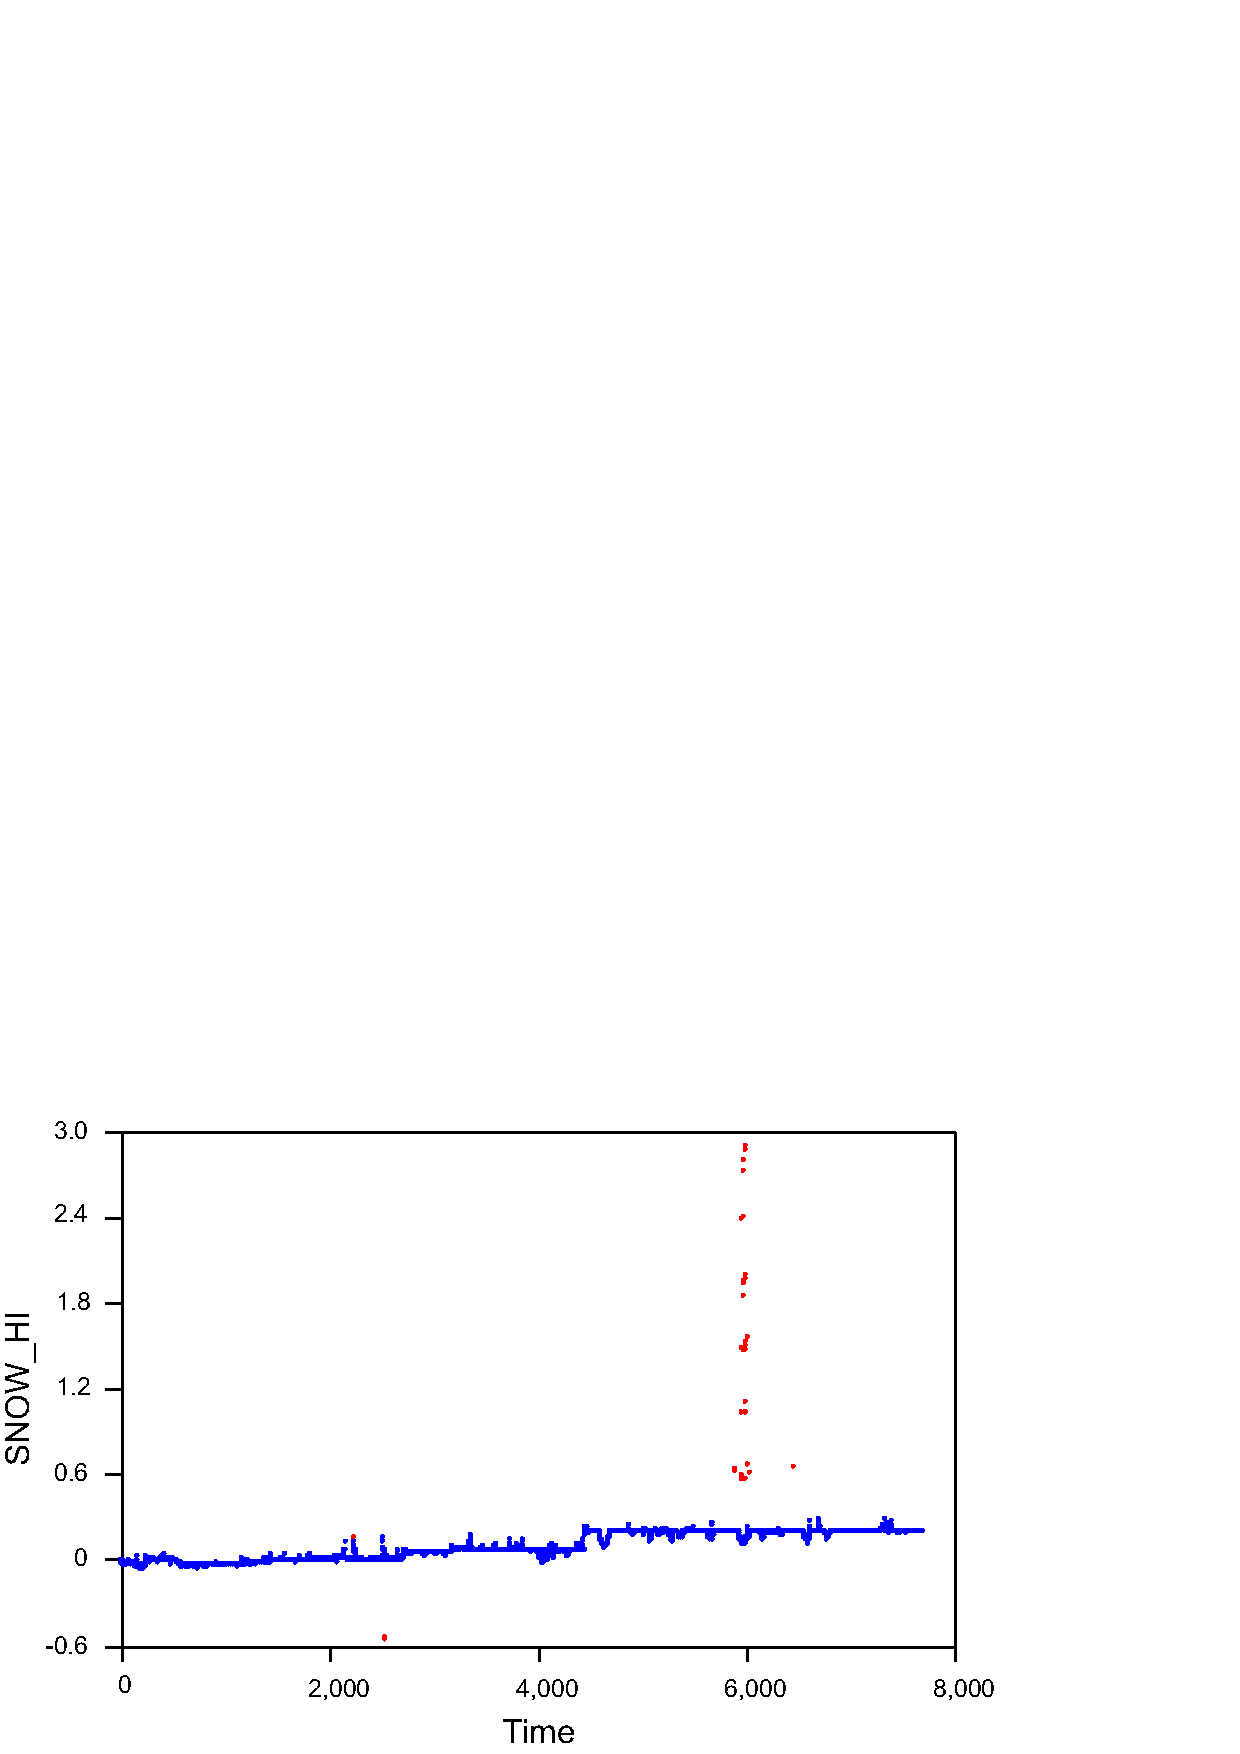
\includegraphics[width=230pt]{figures/snow.pdf}}
\caption{\label{fig:snow}  Outlying measurements of snow cover at a Greenland weather station.}
\end{figure}

\begin{figure}[h]
\centering{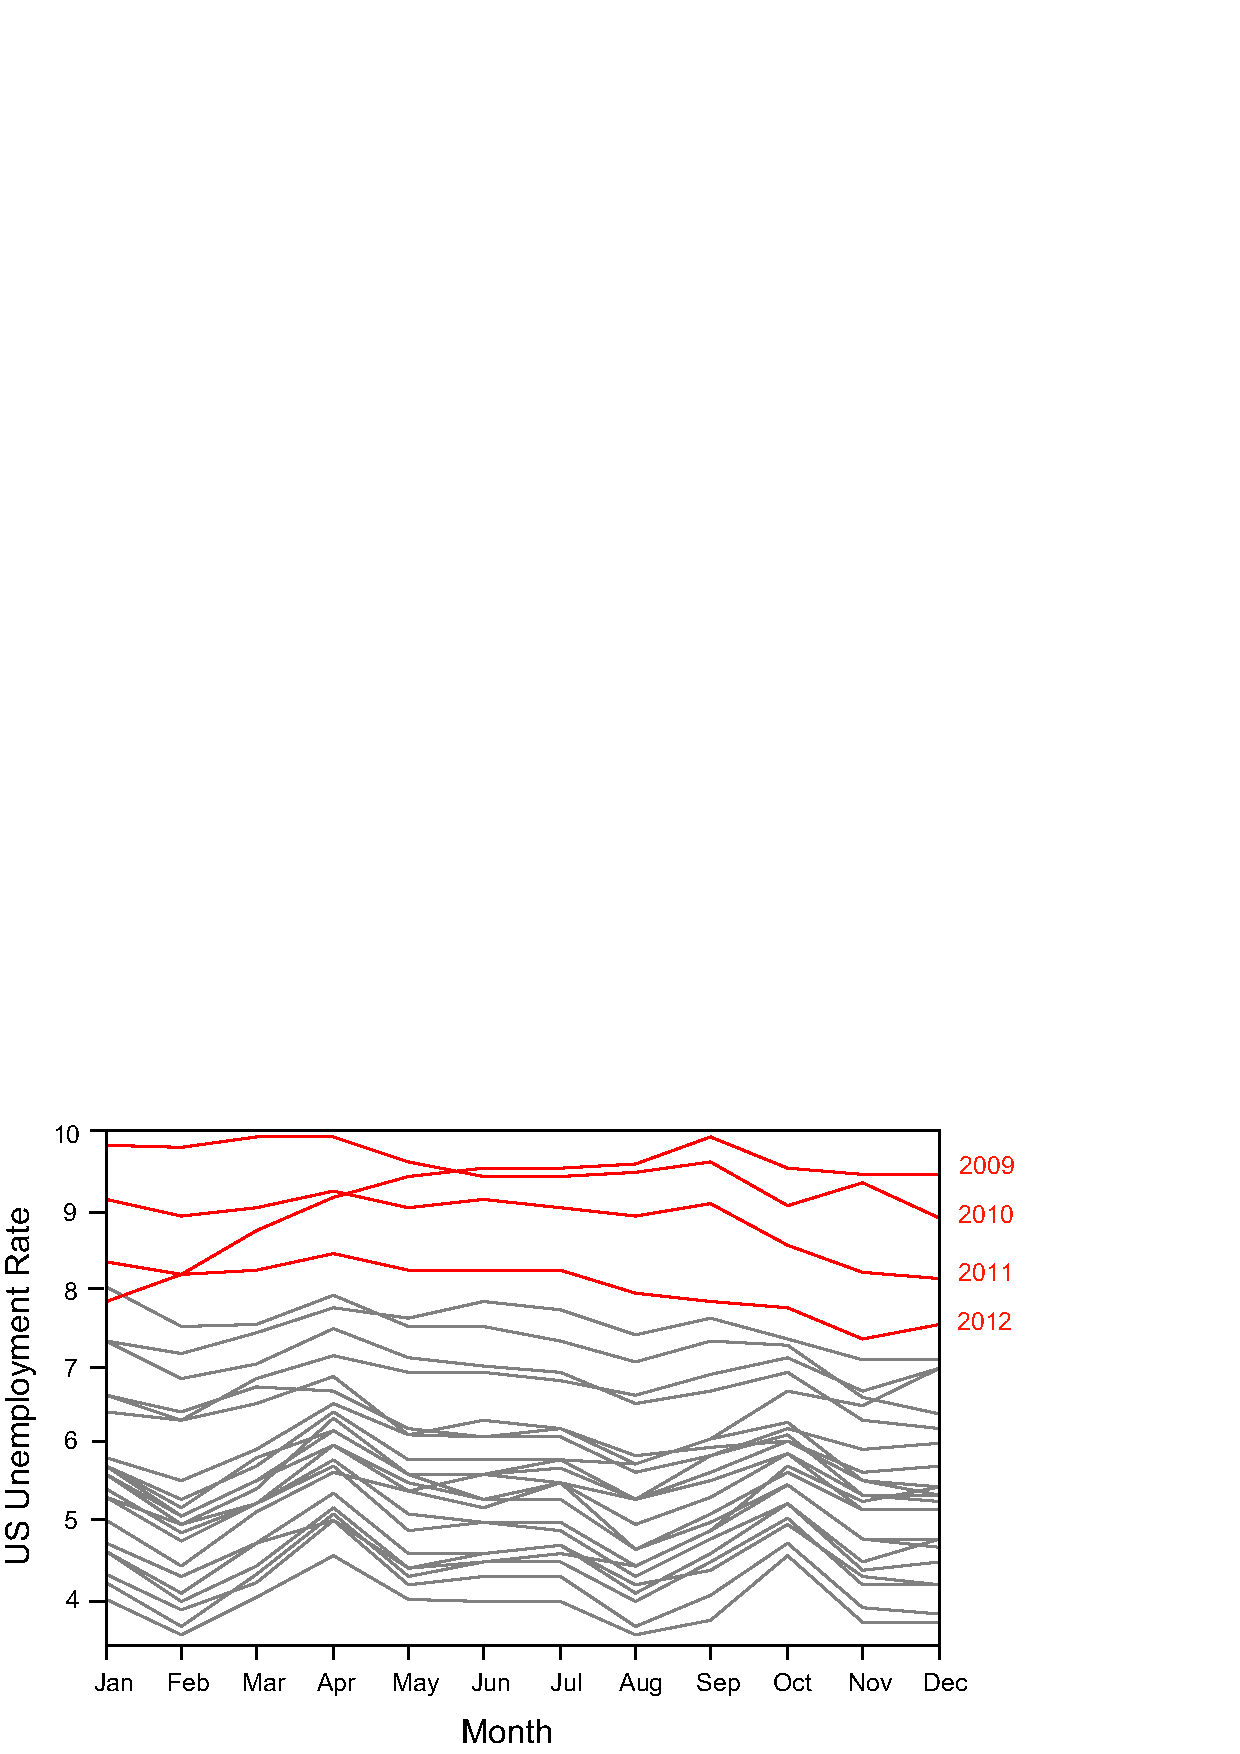
\includegraphics[width=240pt]{figures/USunemployment.pdf}}
\caption{\label{fig:unemployment}  US Unemployment series outliers. The shock and ensuing recovery from the Great Recession is clearly indicated in the outliers.}
\end{figure}

\subsubsection{Ipsative Outliers}
An $ipsative$ outlier is a case that is an outlier with respect to itself. That is, we standardize values within each case (row) and then look for outliers in each standardized profile. Any profile with an outlier identified by $\mathtt{hdoutliers}$ is considered noteworthy; in other words, we can characterize a person simply by referring to his outliers. It is easiest to understand this concept by examining a graphic. Figure~\ref{fig:baseball} shows an outlying profile for a baseball player who is hit by pitches more frequently than we would expect from looking at his other characteristics. This player may not be hit by pitches significantly more than other players, however. We are instead interested in a player with a highly unusual profile that can be described simply by his outlier(s). In every other respect, the player is not necessarily noteworthy. This method should not be used, of course, unless there are enough features to merit computing the statistical outlier model on a case.

\begin{figure}[h]
\centering{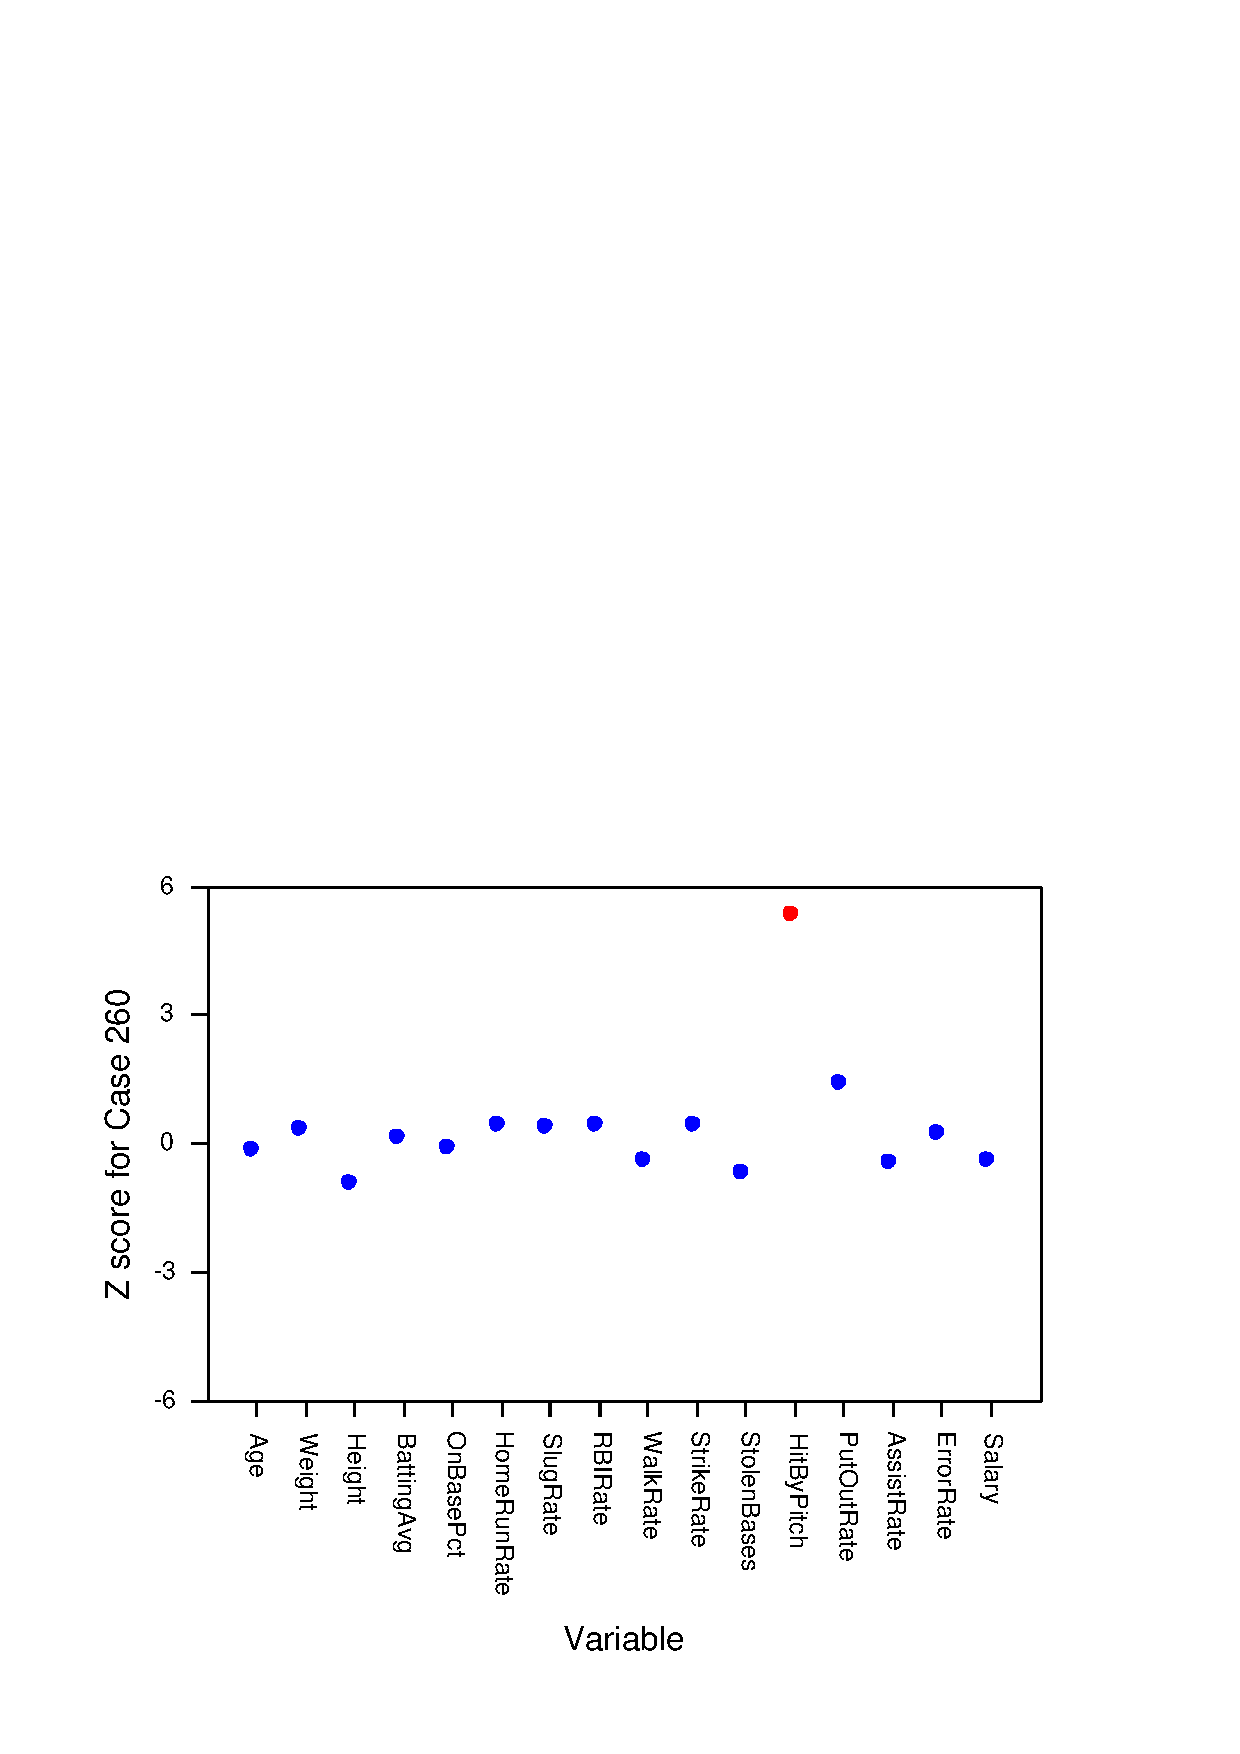
\includegraphics[width=250pt]{figures/baseball.pdf}}
\caption{\label{fig:baseball} One baseball player's profile showing an outlier (hit by pitch) that deviates significantly from his other features.}
\end{figure}


\subsubsection{Text Outliers}
An important application for multivariate outlier detection involves document analysis. Given a collection of documents (Twitter messages, Wikipedia pages, emails, news pages, etc.), one might want to discover any document that is an outlier with respect to the others. The simplest approach to this problem is to use a bag-of-words model. We collect all the words in the documents, stem them to resolve variants, remove stopwords and punctuation, and then apply the tf-idf measure \citep{SaltonTFIDF} on the words within each document. The resulting vectors for each document are then submitted to $\mathtt{hdoutliers}$.

Figure~\ref{fig:novels} shows the results for an analysis of 21 novels from the Guttenberg Web site \citep{Gutenberg}. This problem requires the use of random projections. Before projection, there are 21,021 columns (tf-idf measures) in the dataset. After projection there are 653. Not surprisingly, {\it Ulysses} stands out as an outlier. Distinctively, it contains numerous neologisms. {\it 

Tristram Shandy} was identified by $\mathtt{hdoutliers}$ as the second largest, but not significant, outlier. It too contains numerous neologisms. These two novels lie outside most of the points in Figure~\ref{fig:novels}. Not all multivariate outliers will fall on the periphery of 2D projections, however, as we showed in Section 4.2.

\begin{figure}[h]
\centering{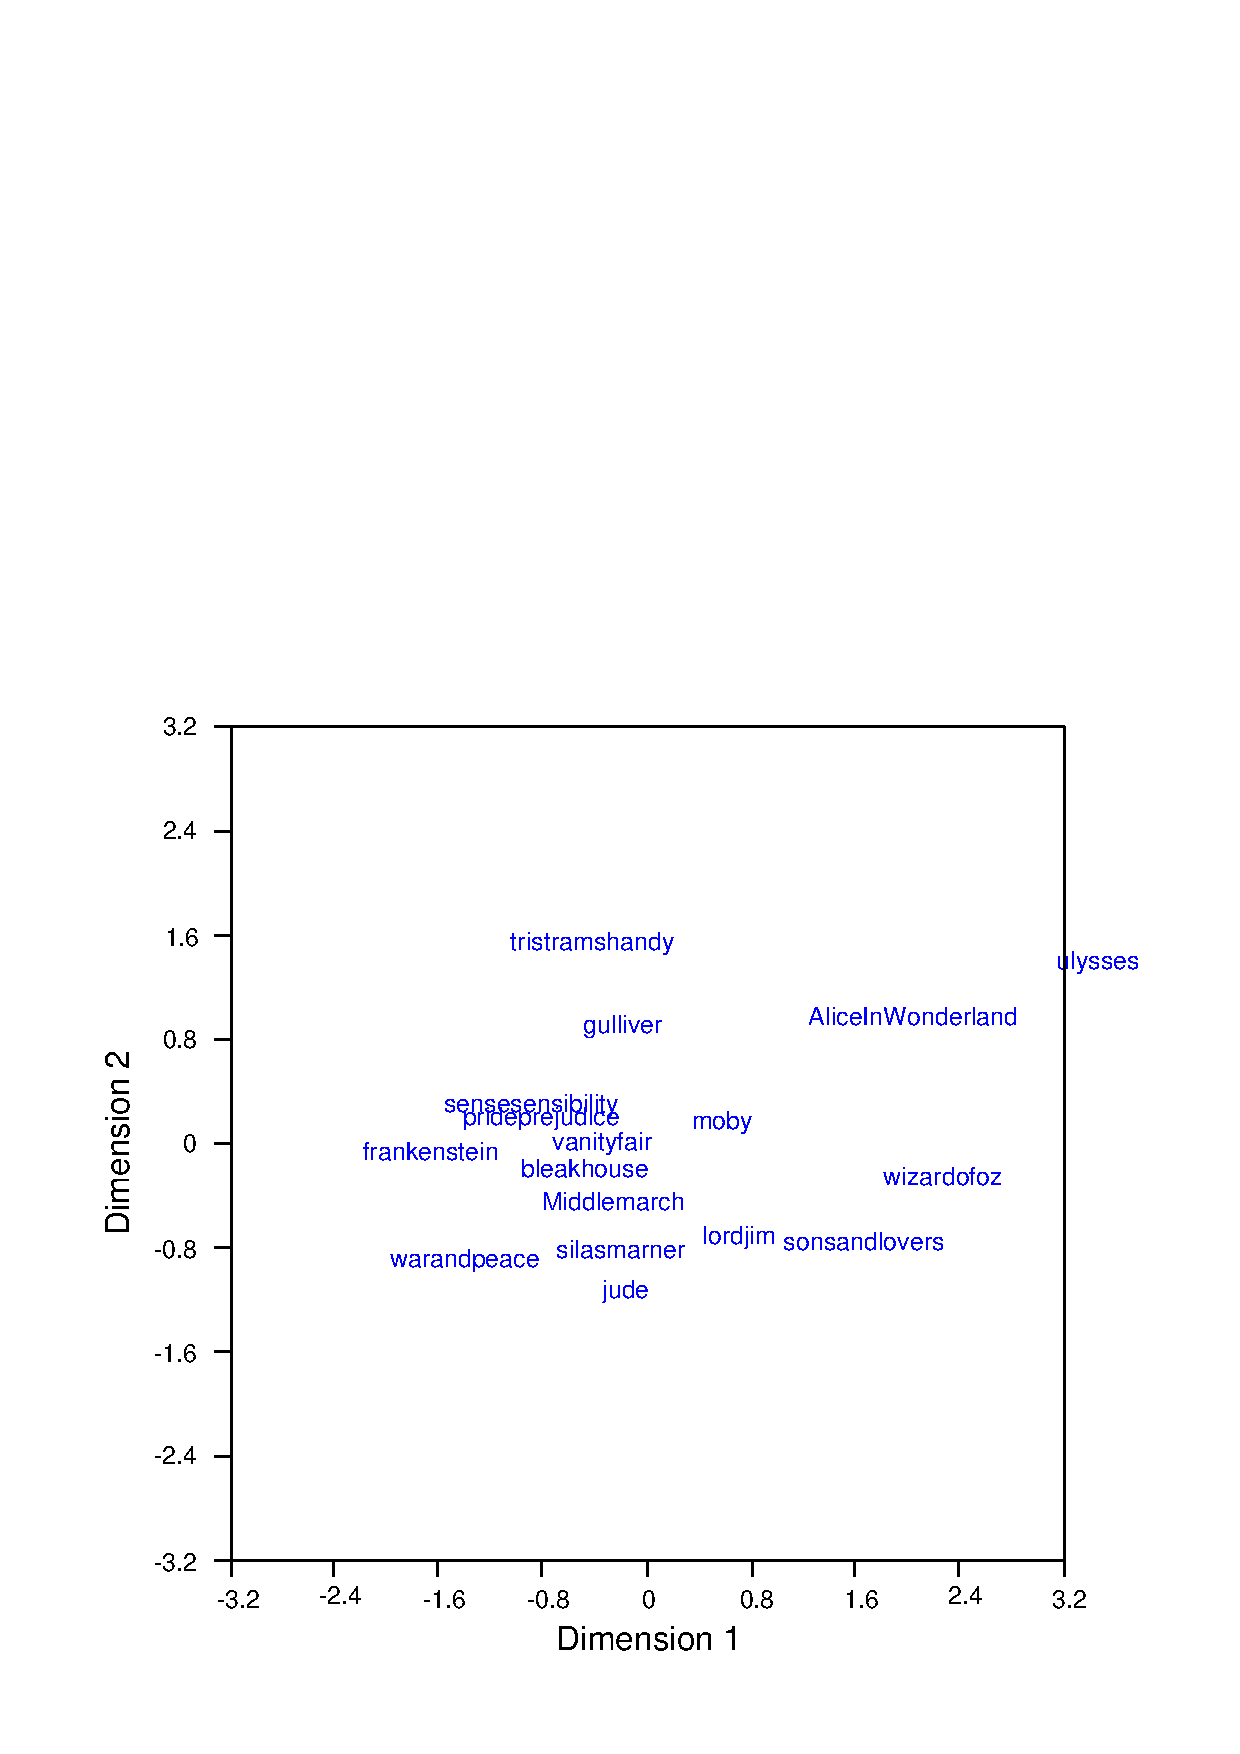
\includegraphics[width=250pt]{figures/novels.pdf}}
\caption{\label{fig:novels}  Document outliers. Nonmetric multidimensional scaling on matrix of Spearman correlations computed on tf-idf scores. The stress for this solution is .163 and one document ({\it Ulysses}) is flagged as an outlier by $\mathtt{hdoutliers}$.}
\end{figure}

\subsection{Graph Outliers}
There are several possibilities related to finding outliers in graphs. One popular application is the discovery of outliers among nodes of a network graph. The best way to exploit $\mathtt{hdoutliers}$ in this context is to featurize the nodes. Common candidates are Prominence, Transitivity (Watts-Strogatz Clustering Coefficient), Closeness Centrality, Betweenness Centrality, Node Degree, Average Degree of Neighbors, and Page Rank \citep{Newman0}. Figure~\ref{fig:lesmis} shows an example for the Les Miserables dataset \citep{StanfordGraphBase}. The nodes were featurized for Betweenness Centrality in order to discover any extraordinarily influential characters. Not surprisingly, Valjean is connected to significantly more characters than anyone else in the book.

\begin{figure}[h]
\centering{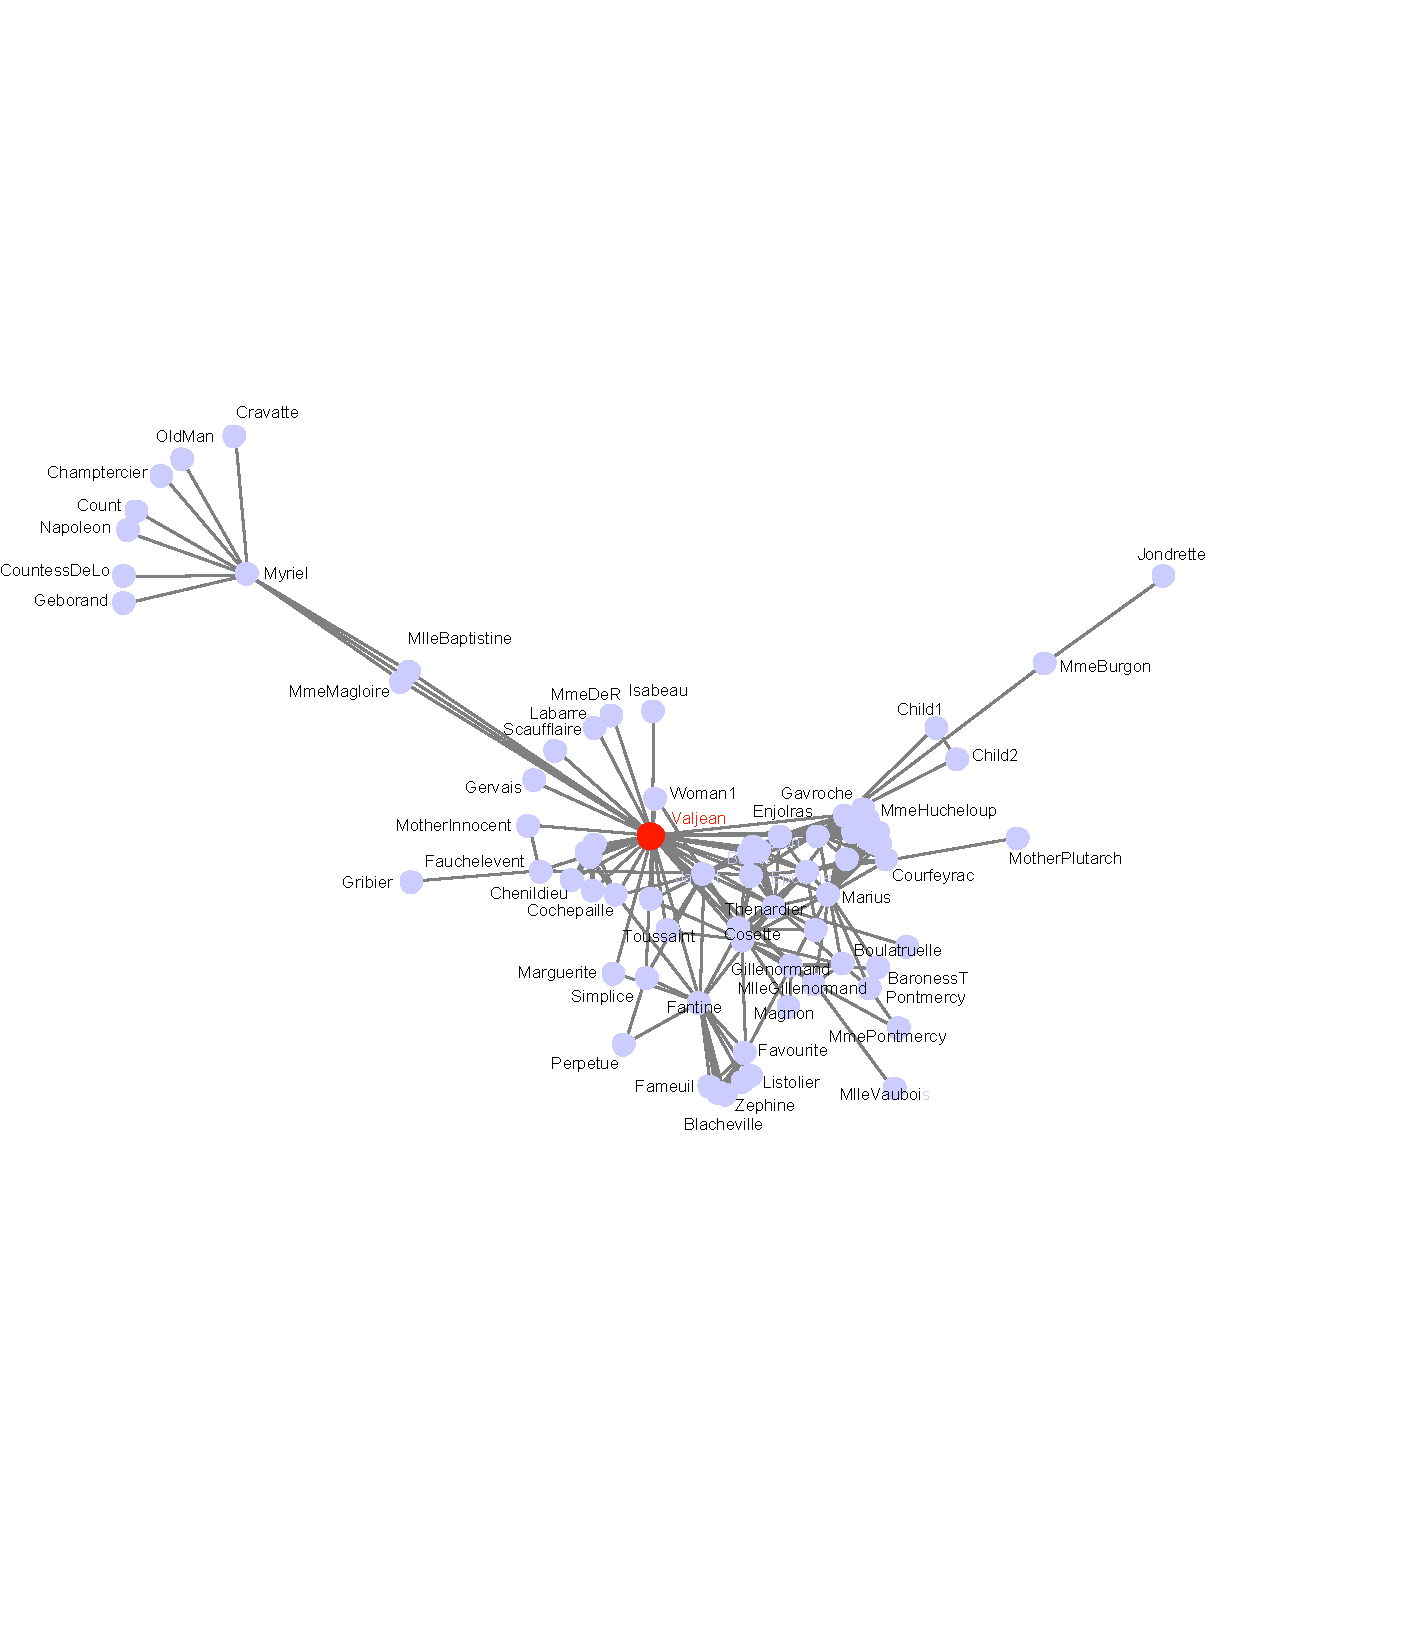
\includegraphics[width=250pt]{figures/lesmis.pdf}}
\caption{\label{fig:lesmis} Les Miserables characters network graph. Valjean is identified as outlying on Betweenness Centrality.}
\end{figure}

An alternative application involves discovering outlying graphs in a collection of graphs. For this problem, we need to find a way to characterize a graph and to derive a distance measure that can be fed to $\mathtt{hdoutliers}$. This application depends on assuming the collection of graphs is derived from a common population model and that any outliers involve a contamination from some alternative model. We need a measure of the distance between two graphs to do this. Unfortunately, graph matching  and related graph edit distance calculations have impractical complexities. Approximate distances are easier to calculate, however \citep{graphMatchingUmeyama}. The approach we take is as follows: 

First, we compute the adjacency matrix for each graph. We then convert the adjacencies above the diagonal to a single binary string. When doing that, however, we have to reorder the adjacency matrix to a canonical form; otherwise, arbitrary input orderings could affect distance calculations on the string. A simple way to do this is to compute the eigendecomposition of the related Laplacian matrix and permute the adjacencies according to the ordering of the values of the eigenvector corresponding to the smallest nonzero eigenvalue. After permuting and encoding the adjacency matrices into strings, we compute the Levenshtein distances \citep{LevenshteinDistance} between pairs of strings. Finally, we assemble the nearest-neighbor distances from the resulting distance matrix and subject them to the $\mathtt{hdoutliers}$ algorithm.

Figure~\ref{fig:graphs} shows an example of this approach using the Karate Club graph \citep{KarateClub}. We generated 15 random minimum spanning tree graphs having the same number of nodes as the Karate Club graph. Then we applied the above procedure to identify outliers. The Karate Club graph was strongly flagged as an outlier by the algorithm.

\begin{figure}[h]
\centering{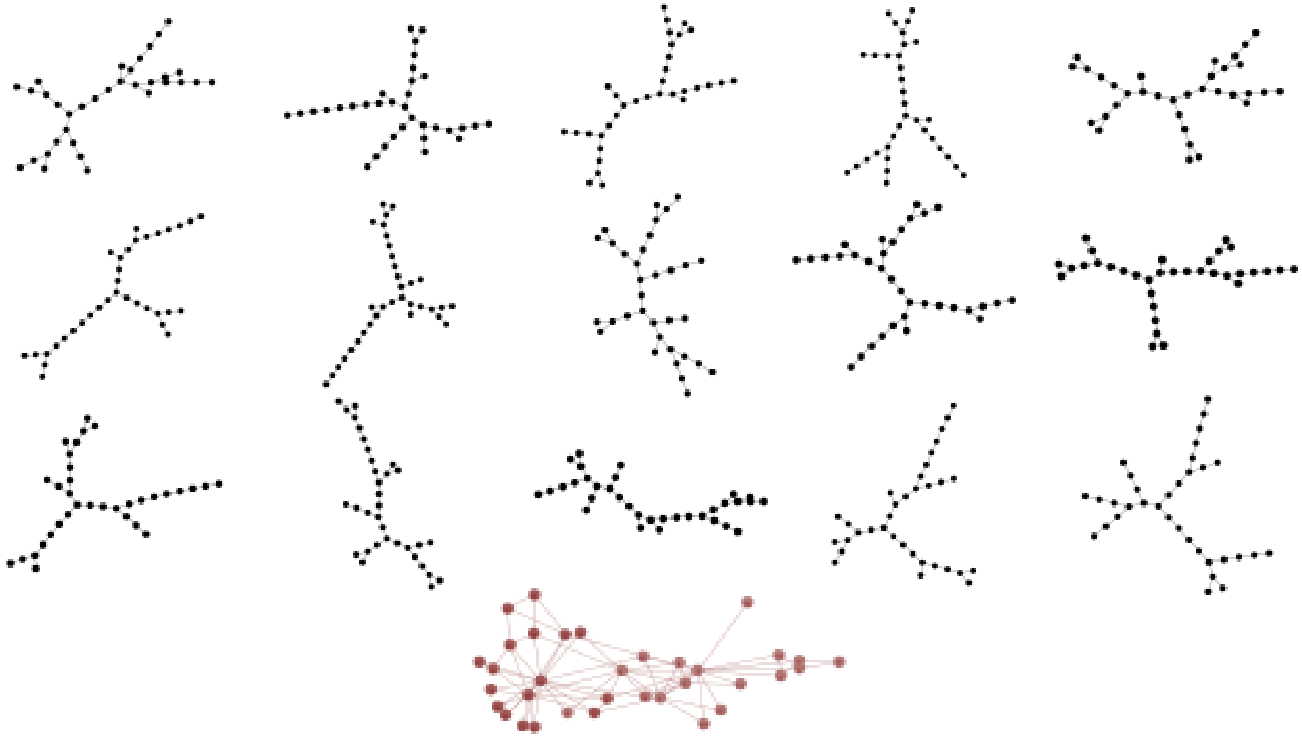
\includegraphics[width=250pt]{figures/karate.pdf}}
\caption{\label{fig:graphs} Karate Club graph (red) is an outlier with respect to comparably scaled random minimum spanning tree graphs.}
\end{figure}


\subsubsection{Scagnostics Outliers}
Scagnostics \citep{Scagnostics} can be used to identify outlying scatterplots. Because the calculations are relatively efficient, these measures can be computed on many thousands of plots in practical time. This outlier application is multivariate, because there are nine scagnostics for each scatterplot, so a multivariate detection algorithm like $\mathtt{hdoutliers}$ is required. 

Figure~\ref{fig:Scagnostics} shows two outlying scatterplots identified by  $\mathtt{hdoutliers}$ when applied to a dataset of baseball player characteristics featured in \cite{ScagnosticsTVCG}. While the left plot in the figure is clearly unusual, the surprising result is to see an evidently bivariate Normal scatterplot of Weight against Height in the right plot. Although the dataset includes many physical and performance features of real baseball players, the type of Normal bivariate distribution found in many introductory statistics books is an outlier among the 120 scatterplots considered in this example. This result should motivate authors writing tutorials on data analysis to include examples beyond Normal distributions.

\begin{figure}[h]
\centering{\includegraphics[width=250pt]{figures/Scagnostics.pdf}}
\caption{\label{fig:Scagnostics} Scatterplot outliers based on Scagnostics computed on 120 scatterplots of baseball player features.}
\end{figure}

\subsubsection{Geographic Outliers}
We can compute spatial outliers using the $\mathtt{hdoutliers}$ algorithm. More frequently, however, maps are a convenient way to display the results of outlier detection on other variables. Figure~\ref{fig:Marriage} shows an example of outlier detection on marriage and divorce rates by US state. Nevada is clearly an outlier.

\begin{figure}[h]
\centering{\includegraphics[width=260pt]{figures/Marriage.pdf}}
\caption{\label{fig:Marriage} Marriage and Divorce rates in the US. There is one state that is an outlier.}
\end{figure}
  

\section{Conclusion}
There is a huge assortment of papers on outlier detection in the statistics and machine learning communities; only a fraction is cited here. While many of the machine learning approaches are ingenious, few rest on a statistical foundation that takes risk into account. If we label something as an outlier, we had better be able to quantify or control our risk.  Methods that do not do this, that simply rank discrepancies or flag observations above an arbitrary threshold (like most machine learning outlier algorithms), can lead to inconsistent results. 

When we do base an algorithm on classical or Bayesian statistical models, however, we have to consider the peculiarities of the many different real datasets that we hope to cover. The $\mathtt{hdoutliers}$ algorithm illustrates some of these considerations. Statisticians can learn from computer scientists how to adapt to unusual or massive data configurations. And computer scientists can learn from statisticians how to incorporate probability into their analytic algorithms.


\bibliographystyle{apalike}
\bibliography{extra/bibliography}
\end{document}

